\section{Sharding}

\subsection{Partición basada en rango}

\begin{figure}[!h]
  \begin{center}
      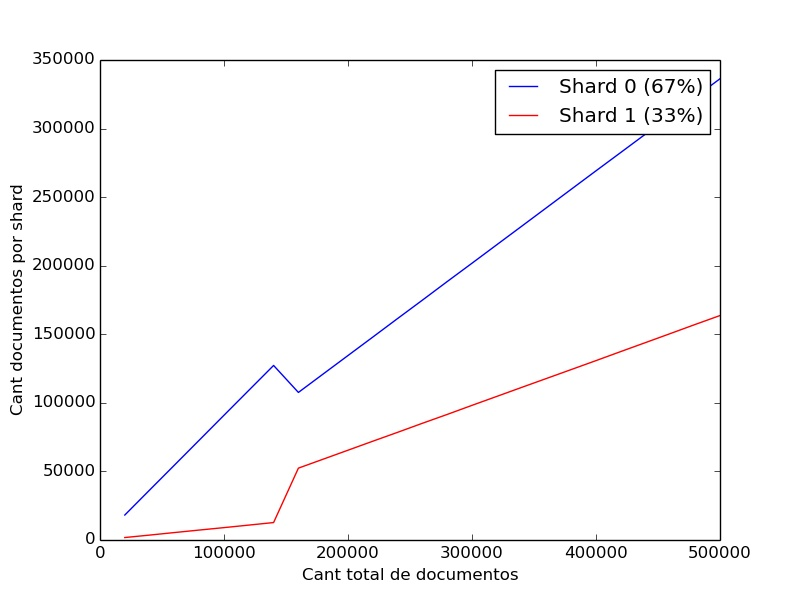
\includegraphics[scale=0.4]{imagenes/range1.jpg}
      \caption{2 Shards utilizando partición de keys por rango}
      \label{fig:contra1}
  \end{center}
\end{figure}

~

\begin{figure}[!h]
  \begin{center}
      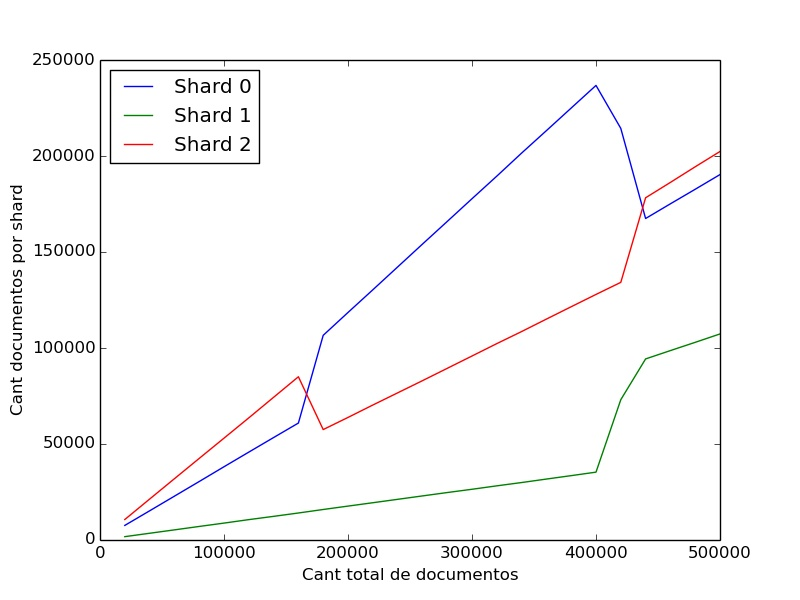
\includegraphics[scale=0.4]{imagenes/range2.jpg}
      \caption{3 Shards utilizando partición de keys por rango}
      \label{fig:contra1}
  \end{center}
\end{figure}

~

\subsection{Partición basada en hash}

\begin{figure}[!h]
  \begin{center}
      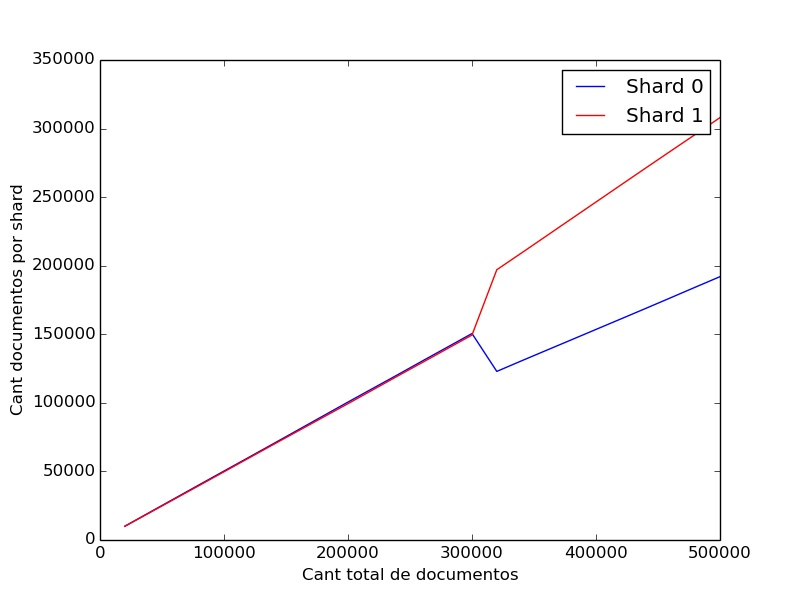
\includegraphics[scale=0.4]{imagenes/hash1.jpg}
      \caption{2 Shards utilizando partición de keys basada en hash}
      \label{fig:contra1}
  \end{center}
\end{figure}

~

\begin{figure}[!h]
  \begin{center}
      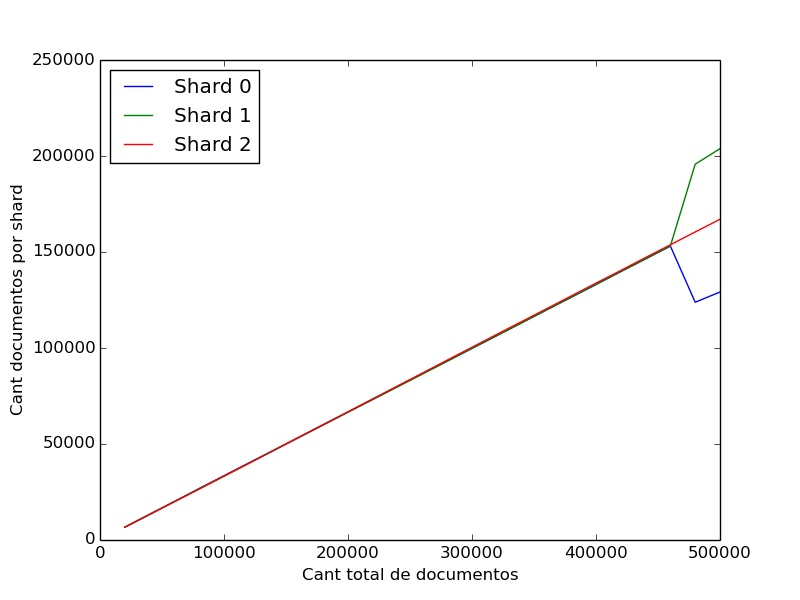
\includegraphics[scale=0.4]{imagenes/hash2.jpg}
      \caption{3 Shards utilizando partición de keys basada en hash}
      \label{fig:contra1}
  \end{center}
\end{figure}

~

